% coding:utf-8

%FOSAET, a LaTeX-Code for a electrical summary of basic electronics
%Copyright (C) 2013, Daniel Winz, Ervin Mazlagic

%This program is free software; you can redistribute it and/or
%modify it under the terms of the GNU General Public License
%as published by the Free Software Foundation; either version 2
%of the License, or (at your option) any later version.

%This program is distributed in the hope that it will be useful,
%but WITHOUT ANY WARRANTY; without even the implied warranty of
%MERCHANTABILITY or FITNESS FOR A PARTICULAR PURPOSE.  See the
%GNU General Public License for more details.
%----------------------------------------

\chapter{Schaltungstechnik}
\newpage
% coding:utf-8

%FOSAET, a LaTeX-Code for a electrical summary of basic electronics
%Copyright (C) 2013, Daniel Winz, Ervin Mazlagic

%This program is free software; you can redistribute it and/or
%modify it under the terms of the GNU General Public License
%as published by the Free Software Foundation; either version 2
%of the License, or (at your option) any later version.

%This program is distributed in the hope that it will be useful,
%but WITHOUT ANY WARRANTY; without even the implied warranty of
%MERCHANTABILITY or FITNESS FOR A PARTICULAR PURPOSE.  See the
%GNU General Public License for more details.
%----------------------------------------

\section{Spannungsteiler}

\subsection{unbelasteter Spannungsteiler}
\begin{figure}[h!]
	\centering
	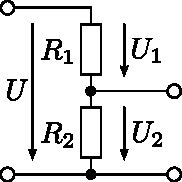
\includegraphics[scale=\schscale]{uteil.pdf}
	\caption{unbelasteter Spannungsteiler}
	\label{sch:uteil}
\end{figure}
\[ U_2 = \frac{U_1}{R_1 + R_2} \cdot R_2 \]

\subsection{belasteter Spannungsteiler}
\begin{figure}[h!]
	\centering
	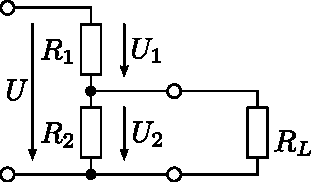
\includegraphics[scale=\schscale]{uteilbel.pdf}
	\caption{belasteter Spannungsteiler}
	\label{sch:uteilbel}
\end{figure}
\[ U_2 = \frac{U_1}{R_1 + \frac{R_2 \cdot R_L}{R_2 + R_L}} \cdot \frac{R_2 \cdot R_L}{R_2 + R_L} \]

\newpage
\subsection{unbelastetes Potentiometer}
\begin{figure}[h!]
	\centering
	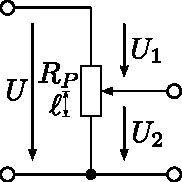
\includegraphics[scale=\schscale]{poti.pdf}
	\caption{unbelastetes Potentiometer}
	\label{sch:poti}
\end{figure}
\[ U_2 = U_1 \cdot \ell \]

\subsection{belastetes Potentiometer}
\begin{figure}[h!]
	\centering
	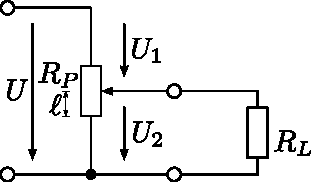
\includegraphics[scale=\schscale]{potibel.pdf}
	\caption{belastetes Potentiometer}
	\label{sch:potibel}
\end{figure}
\[ U_2 = \frac{U_1}{R_p \cdot (1 - \ell) + \frac{R_p \cdot \ell \cdot R_L}{R_p \cdot \ell + R_L}} \cdot \frac{R_p \cdot \ell \cdot R_L}{R_p \cdot \ell + R_L} \]
       % Spannungsteiler
% coding:utf-8

%FOSAET, a LaTeX-Code for a electrical summary of basic electronics
%Copyright (C) 2013, Daniel Winz, Ervin Mazlagic

%This program is free software; you can redistribute it and/or
%modify it under the terms of the GNU General Public License
%as published by the Free Software Foundation; either version 2
%of the License, or (at your option) any later version.

%This program is distributed in the hope that it will be useful,
%but WITHOUT ANY WARRANTY; without even the implied warranty of
%MERCHANTABILITY or FITNESS FOR A PARTICULAR PURPOSE.  See the
%GNU General Public License for more details.
%----------------------------------------

\section{Stromteiler}
\begin{figure}[h!]
	\centering
	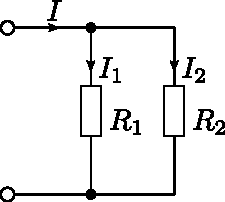
\includegraphics[scale=\schscale]{iteil.pdf}
	\caption{Stromteiler}
	\label{sch:iteil}
\end{figure}
\[ I_2 = I \cdot \frac{R_1}{R_1 + R_2} \]

\subsubsection{Stromteiler mit $> 2$ Widerständen}
\[ I_n = I_q \cdot \frac{(R1 // R2 \dots // R_{n-1})}
{(R1 // R2 \dots // R_{n-1}) + R_n} 
= I_q \cdot \frac{\left(\frac{R_1 \cdot R_2 \dots R_{n-1}}
{R_1 + R_2 \dots R_{n-1}}\right)}
{\left(\frac{R_1 \cdot R_2 \dots R_{n-1}}
{R_1 + R_2 \dots R_{n-1}}\right) + R_n} \]       % Stromteiler
% coding:utf-8

%FOSAET, a LaTeX-Code for a electrical summary of basic electronics
%Copyright (C) 2013, Daniel Winz, Ervin Mazlagic

%This program is free software; you can redistribute it and/or
%modify it under the terms of the GNU General Public License
%as published by the Free Software Foundation; either version 2
%of the License, or (at your option) any later version.

%This program is distributed in the hope that it will be useful,
%but WITHOUT ANY WARRANTY; without even the implied warranty of
%MERCHANTABILITY or FITNESS FOR A PARTICULAR PURPOSE.  See the
%GNU General Public License for more details.
%----------------------------------------

\newpage
\section{Brückenschaltung}
\begin{figure}[h!]
  \centering
  \begin{circuitikz}[scale=1]\draw
    (1.5,6) to[short, o-*] (1.5,5)
    (1.5,1) to[short, *-o] (1.5,0)
    (0,5) to[short, ] (3,5)
    (0,1) to[short, ] (3,1)
    (0,5) to[R=$R_1$, ] (0,3)
    (0,3) to[R=$R_2$, ] (0,1)
    (3,5) to[R=$R_3$, ] (3,3)
    (3,3) to[R=$R_4$, ] (3,1)
    (0,3) to[R=$R_5$, *-*] (3,3)
    ;
  \end{circuitikz}
  \caption{Brückenschaltung}
\end{figure}

\subsubsection{Abgeglichene Brückenschaltung}
\[ \frac{R_1}{R_2} = \frac{R_3}{R_4} \]
\[ U_5 = U_2 - U_4 = 0 \]
\[ I_5 = 0 \]

\subsubsection{Nicht abgegelichen ohne $R_5$}
\[ U_5 = U_2 - U_4 = U_q \cdot \left( \left( \frac{R_2}{R_1 + R_2} \right) - 
\left( \frac{R_4}{R_3 + R_4} \right) \right) \]

\subsubsection{Nicht abgeglichen}
\begin{scriptsize}
\[ U_5 = U_q \cdot \frac{(R_2 \cdot R_3 - R_1 \cdot R_4) \cdot R_5}
{R_5 \cdot (R_3 + R_4) \cdot (R_1 + R_2) 
+ R_1 \cdot R_3 \cdot R_4 + R_2 \cdot R_3 \cdot R_4 
+ R_1 \cdot R_2 \cdot R_3 + R_1 \cdot R_2 \cdot R_4} \]
\[ I_5 = U_q \cdot \frac{R_2 \cdot R_3 - R_1 \cdot R_4}
{R_5 \cdot (R_3 + R_4) \cdot (R_1 + R_2) 
+ R_3 \cdot R_4 \cdot (R_1 + R_2) + R_1 \cdot R_2 \cdot (R_3 + R_4)} \]
\end{scriptsize}      % Brückenschaltung
% coding:utf-8

%FOSAET, a LaTeX-Code for a electrical summary of basic electronics
%Copyright (C) 2013, Daniel Winz, Ervin Mazlagic

%This program is free software; you can redistribute it and/or
%modify it under the terms of the GNU General Public License
%as published by the Free Software Foundation; either version 2
%of the License, or (at your option) any later version.

%This program is distributed in the hope that it will be useful,
%but WITHOUT ANY WARRANTY; without even the implied warranty of
%MERCHANTABILITY or FITNESS FOR A PARTICULAR PURPOSE.  See the
%GNU General Public License for more details.
%----------------------------------------

\section{Leistungsanpassung}
Soll einer Quelle die maximal mögliche Leistung entnommen werden, so wird 
Leistungsanpassung vorgenommen. Bei Leistungsanpassung entspricht der Wert des 
Lastwiderstandes demjenigen des Innenwiderstandes der Quelle. 
\[ R_L = R_i \]
\[ P = \frac{\frac{U_q}{2}}{R_l} \]

\subsubsection{Leistungsanpassung bei komplexen Impedanzen}
$R_L$ Real: 
\[ R_L = ||Z_i|| \]
$Z_L$ Komplex: 
\[ Z_L = {Z_i}^* \]      % Leistungsanpassung
% coding:utf-8

%FOSAET, a LaTeX-Code for a electrical summary of basic electronics
%Copyright (C) 2013, Daniel Winz, Ervin Mazlagic

%This program is free software; you can redistribute it and/or
%modify it under the terms of the GNU General Public License
%as published by the Free Software Foundation; either version 2
%of the License, or (at your option) any later version.

%This program is distributed in the hope that it will be useful,
%but WITHOUT ANY WARRANTY; without even the implied warranty of
%MERCHANTABILITY or FITNESS FOR A PARTICULAR PURPOSE.  See the
%GNU General Public License for more details.
%----------------------------------------

\newpage
\section{Umwandlung Spannungsquelle $\leftrightarrow$ Stromquelle}

\subsection{Thévenin-Theorem}
Nach Thévenin kann jedes Netzwerk bestehend aus Strom-, Spannungsquellen und Widerständen in eine Ersatzspannungsquelle\footnote{Thévenin-Äquivalent} gewandelt werden.

\begin{figure}[h!]
\centering
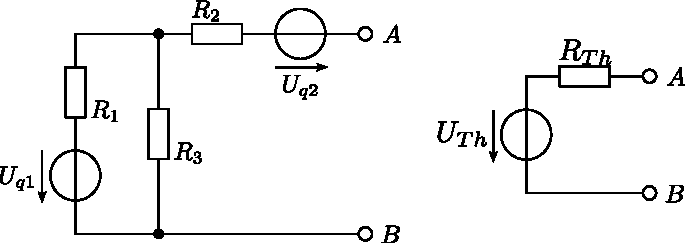
\includegraphics[scale=\schscale]{thevenin_sch_2.pdf}
\caption{Schaltung (l) und ihr Thévenin-Äquivalent (r)}
\label{sch:thevenin}
\end{figure}

\subsubsection{Berechnung}
\begin{itemize}
\item Leerlaufspannung $U_{Th}$ bestimmen (siehe Kapitel~\ref{sec:superpos})
\item Ersatzwiderstand ermitteln durch ausschalten aller unabhängiger Quellen (Spannungsquellen werden kurzgeschlossen, Stromquellen unterbrochen)
\end{itemize}

\newpage
\subsection{Norton-Theorem}
Nach Norton kann jedes Netzwerk bestehend aus Strom-, Spannungsquellen und Widerständen in eine Ersatzstromquelle\footnote{Norton-Äqivalent} gewandelt werden.

\begin{figure}[h!]
\centering
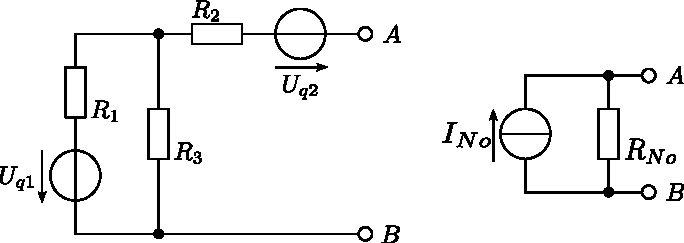
\includegraphics[scale=\schscale]{norton_sch_2.pdf}
\caption{Schaltung (l) und ihr Norton-Äquivalent (r)}
\label{sch:norton}
\end{figure}

\subsection{Spannungsquelle $\rightarrow$ Stromquelle}
\[ R_{No} = R_{Th} \]
\[ I_q = \frac{U_q}{R_{Th}} \]

\subsection{Stromquelle $\rightarrow$ Spannungsquelle}
\[ R_{Th} = R_{No} \]
\[ U_q = I_q \cdot R_{No} \]
    % Umwandlung Spannungsquelle <-> Stromquelle
% coding:utf-8

%FOSAET, a LaTeX-Code for a electrical summary of basic electronics
%Copyright (C) 2013, Daniel Winz, Ervin Mazlagic

%This program is free software; you can redistribute it and/or
%modify it under the terms of the GNU General Public License
%as published by the Free Software Foundation; either version 2
%of the License, or (at your option) any later version.

%This program is distributed in the hope that it will be useful,
%but WITHOUT ANY WARRANTY; without even the implied warranty of
%MERCHANTABILITY or FITNESS FOR A PARTICULAR PURPOSE.  See the
%GNU General Public License for more details.
%----------------------------------------

\section{Umwandlung Stern $\leftrightarrow$ Dreieck}
\begin{figure}[h!]
	\centering
	\begin{subfigure}[b]{0.4\textwidth}
		\centering
		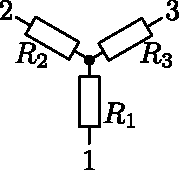
\includegraphics[scale=\schscale]{star_sch.pdf}
		\caption{Sternschaltung}
		\label{sch:star}
	\end{subfigure}
	\begin{subfigure}[b]{0.4\textwidth}
		\centering
		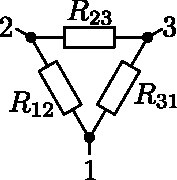
\includegraphics[scale=\schscale]{tri_sch.pdf}
		\caption{Dreieckschaltung}
		\label{sch:tri}
	\end{subfigure}
	\caption{Stern und Dreieckschaltung}
	\label{sch:tristar}
\end{figure}


\subsection{Umwandlung Dreieck $\to$ Stern}
\[ \begin{matrix}
R_1 = \dfrac{R_{12} \cdot R_{31}}{R_{12} + R_{23} + R_{31}}\\\\
R_2 = \dfrac{R_{23} \cdot R_{12}}{R_{12} + R_{23} + R_{31}}\\\\
R_3 = \dfrac{R_{31} \cdot R_{23}}{R_{12} + R_{23} + R_{31}}\\\\
\end{matrix} \]

\subsection{Umwandlung Stern $\to$ Dreieck}
\[ \begin{matrix}
R_{12} = \dfrac{R_1 \cdot R_2 + R_2 \cdot R_3 + R_3 \cdot R_1}{R_3}\\\\
R_{23} = \dfrac{R_1 \cdot R_2 + R_2 \cdot R_3 + R_3 \cdot R_1}{R_1}\\\\
R_{31} = \dfrac{R_1 \cdot R_2 + R_2 \cdot R_3 + R_3 \cdot R_1}{R_2}\\\\
\end{matrix} \]

\subsection{Umwandlung Dreieck $\to$ Stern mit identischen Widerständen}
\[ R_{\upY} = \frac{R_{\triangle}}{3} \]

\subsection{Umwandlung Stern $\to$ Dreieck mit identischen Widerständen}
\[ R_{\triangle} = 3 \cdot R_{\upY} \]     % Dreieck <-> Stern Umwandlung
% coding:utf-8

%FOSAET, a LaTeX-Code for a electrical summary of basic electronics
%Copyright (C) 2013, Daniel Winz, Ervin Mazlagic

%This program is free software; you can redistribute it and/or
%modify it under the terms of the GNU General Public License
%as published by the Free Software Foundation; either version 2
%of the License, or (at your option) any later version.

%This program is distributed in the hope that it will be useful,
%but WITHOUT ANY WARRANTY; without even the implied warranty of
%MERCHANTABILITY or FITNESS FOR A PARTICULAR PURPOSE.  See the
%GNU General Public License for more details.
%----------------------------------------

\section{Quellenvereinfachung}
Interessiert die Leistung an der Quelle nicht oder ist die Spannung an 
Stromquellen oder der Strom durch Spannungsquellen nicht wichtig, können 
Quellen wie folgt vereinfacht werden. 
\begin{center}
\begin{minipage}[c]{0.3\textwidth}
\begin{circuitikz}[scale=1]\draw
  (0,5) to[V=$U_q$, o-] (0,3)
  (0,3) to[I=$I_q$, -o] (0,1)
  ;
\end{circuitikz}
\end{minipage}
\begin{minipage}[c]{0.1\textwidth}
\Huge$\Rightarrow$
\end{minipage}
\begin{minipage}[c]{0.3\textwidth}
\begin{circuitikz}[scale=1]\draw
  (2,4) to[I=$I_q$, o-o] (2,2)
  ;
\end{circuitikz}
\end{minipage}
\end{center}
%
\begin{center}
\begin{minipage}[c]{0.3\textwidth}
\begin{circuitikz}[scale=1]\draw
  (1,4) to[short, o-*] (1,3)
  (0,3) to[short, ] (2,3)
  (0,1) to[short, ] (2,1)
  (1,1) to[short, *-o] (1,0)
  (0,3) to[V=$U_q$, ] (0,1)
  (2,3) to[I=$I_q$, ] (2,1)
  ;
\end{circuitikz}
\end{minipage}
\begin{minipage}[c]{0.1\textwidth}
\Huge$\Rightarrow$
\end{minipage}
\begin{minipage}[c]{0.3\textwidth}
\begin{circuitikz}[scale=1]\draw
  (4,3) to[V=$U_q$, o-o] (4,1)
  ;
\end{circuitikz}
\end{minipage}
\end{center}
%
\begin{center}
\begin{minipage}[c]{0.3\textwidth}
\begin{circuitikz}[scale=1]\draw
  (0,5) to[R=$R$, o-] (0,3)
  (0,3) to[I=$I_q$, -o] (0,1)
  ;
\end{circuitikz}
\end{minipage}
\begin{minipage}[c]{0.1\textwidth}
\Huge$\Rightarrow$
\end{minipage}
\begin{minipage}[c]{0.3\textwidth}
\begin{circuitikz}[scale=1]\draw
  (2,4) to[I=$I_q$, o-o] (2,2)
  ;
\end{circuitikz}
\end{minipage}
\end{center}
%
\begin{center}
\begin{minipage}[c]{0.3\textwidth}
\begin{circuitikz}[scale=1]\draw
  (1,4) to[short, o-*] (1,3)
  (0,3) to[short, ] (2,3)
  (0,1) to[short, ] (2,1)
  (1,1) to[short, *-o] (1,0)
  (0,3) to[V=$U_q$, ] (0,1)
  (2,3) to[R=$R$, ] (2,1)
  ;
\end{circuitikz}
\end{minipage}
\begin{minipage}[c]{0.1\textwidth}
\Huge$\Rightarrow$
\end{minipage}
\begin{minipage}[c]{0.3\textwidth}
\begin{circuitikz}[scale=1]\draw
  (4,3) to[V=$U_q$, o-o] (4,1)
  ;
\end{circuitikz}
\end{minipage}
\end{center}
%
       % Quellenvereinfachung
% coding:utf-8

%FOSAET, a LaTeX-Code for a electrical summary of basic electronics
%Copyright (C) 2013, Daniel Winz, Ervin Mazlagic

%This program is free software; you can redistribute it and/or
%modify it under the terms of the GNU General Public License
%as published by the Free Software Foundation; either version 2
%of the License, or (at your option) any later version.

%This program is distributed in the hope that it will be useful,
%but WITHOUT ANY WARRANTY; without even the implied warranty of
%MERCHANTABILITY or FITNESS FOR A PARTICULAR PURPOSE.  See the
%GNU General Public License for more details.
%----------------------------------------

\newpage
\section{Quellenverschiebung}
Das Verschieben von Quellen kann notwendig sein, wenn zum Beispiel beim Knotenpotentialverfahren eine ideale Spannungsquelle nicht in eine Stromquelle umgewandelt werden kann. 

\subsection{Verschiebung von Spannungsquellen}
\begin{enumerate}
  \item Knoten bestimmen, über welchen die Spannungsquelle verschoben werden soll. 
  \item Spannungsquelle vervielfachen und über Knoten verschieben. \\
  Dabei muss die Spannungsquelle auf jede Leitung verschoben werden, welche zum Knoten führt. Somit werden die Maschengleichungen nicht verändert. 
\end{enumerate}
% Spannungsquellen können über einen Knoten hinweg geschoben werden. Bei der Verschiebung muss er vervielfacht werden und auf jede andere Leitung am Knoten eingefügt werden. 
\begin{figure}[h!]
	\centering
	\begin{subfigure}[b]{0.4\textwidth}
		\centering
		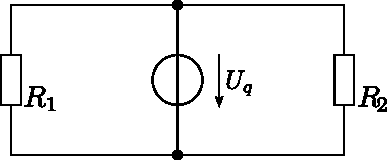
\includegraphics[scale=\schscalesmall]{../fig/qversch_uq1_sch.pdf}
% 		\caption{1}
		\label{sch:starqversch_uq1}
	\end{subfigure}
	\begin{subfigure}[b]{0.4\textwidth}
		\centering
		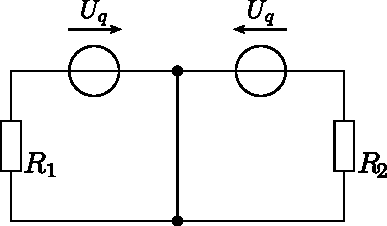
\includegraphics[scale=\schscalesmall]{../fig/qversch_uq2_sch.pdf}
% 		\caption{2}
		\label{sch:qversch_uq2}
	\end{subfigure}
	\caption{Verschiebung von Spannungsquellen}
	\label{sch:qversch_uq1}
\end{figure}

\newpage
\subsection{Verschiebung von Stromquellen}
\begin{enumerate}
  \item Masche bestimmen, innerhalb welcher die Stromquelle verschoben werden soll. 
  \item Stromquelle vervielfachen. 
  \item Stromquellen verschieben, dass zwischen jedem Knoten ausser an der Stelle der vorherigen Stromquelle eine Stromquelle zu liegen kommt. 
\end{enumerate}
% Stromquellen werden zunächst vervielfacht und anschliessend innerhalb der Masche an jeden Knoten "umgehängt". 
\begin{figure}[h!]
	\centering
	\begin{subfigure}[b]{0.3\textwidth}
		\centering
		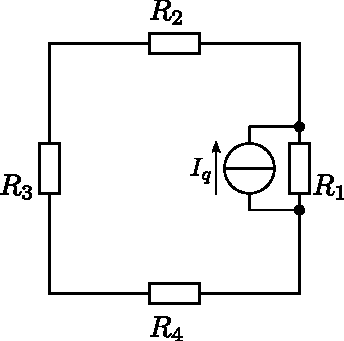
\includegraphics[scale=\schscalesmall]{../fig/qversch_iq1_sch.pdf}
% 		\caption{1}
		\label{sch:qversch_iq1}
	\end{subfigure}
	\begin{subfigure}[b]{0.3\textwidth}
		\centering
		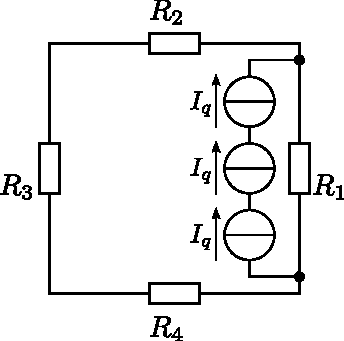
\includegraphics[scale=\schscalesmall]{../fig/qversch_iq2_sch.pdf}
% 		\caption{2}
		\label{sch:qversch_iq2}
	\end{subfigure}
	\begin{subfigure}[b]{0.3\textwidth}
		\centering
		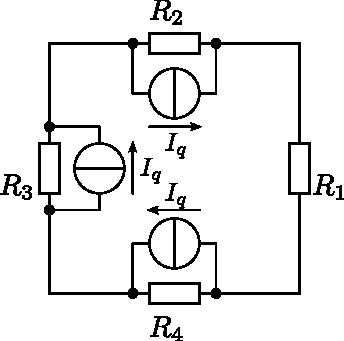
\includegraphics[scale=\schscalesmall]{../fig/qversch_iq3_sch.pdf}
% 		\caption{3}
		\label{sch:qversch_iq3}
	\end{subfigure}
	\caption{Verschiebung von Stromquellen}
	\label{sch:qversch_iq}
\end{figure}
     % Quellenverschiebung
% coding:utf-8

%FOSAET, a LaTeX-Code for a electrical summary of basic electronics
%Copyright (C) 2013, Daniel Winz, Ervin Mazlagic

%This program is free software; you can redistribute it and/or
%modify it under the terms of the GNU General Public License
%as published by the Free Software Foundation; either version 2
%of the License, or (at your option) any later version.

%This program is distributed in the hope that it will be useful,
%but WITHOUT ANY WARRANTY; without even the implied warranty of
%MERCHANTABILITY or FITNESS FOR A PARTICULAR PURPOSE.  See the
%GNU General Public License for more details.
%----------------------------------------

\section{Superposition}
\label{sec:superpos}
Unter Superposition bzw. Überlagerung versteht man, dass gleiche Grössen sich linear überlagern.
In der Elektrotechnik z.B. bei der bestimmung von Netzwerkspannungen. 
So kann ein Netzwerk mit mehreren Quellen per Superposition einfach analysiert werden, indem man das Netzwerk mit jeweils einer aktiver Quelle betrachtet. 
Unabhängige Spannungsquellen werden kurzgeschlossen und unabhängige Stromquellen unterbrochen.
Die Ergenisse jeder Betrachtung können dann linear kombiniert bzw. überlagert werden.
    % Superposition bzw. Überlagerung
% coding:utf-8

%FOSAET, a LaTeX-Code for a electrical summary of basic electronics
%Copyright (C) 2013, Daniel Winz, Ervin Mazlagic

%This program is free software; you can redistribute it and/or
%modify it under the terms of the GNU General Public License
%as published by the Free Software Foundation; either version 2
%of the License, or (at your option) any later version.

%This program is distributed in the hope that it will be useful,
%but WITHOUT ANY WARRANTY; without even the implied warranty of
%MERCHANTABILITY or FITNESS FOR A PARTICULAR PURPOSE.  See the
%GNU General Public License for more details.
%----------------------------------------

\newpage
\section{Knotenpotentialverfahren}
\begin{enumerate}
  \item Alle realen Spannungsquellen in Stromquellen umwandeln. 
  \item Null-Potential ($N_0$) wählen (bestenfalls dort wo der Strom gesucht ist)
  \item restliche Knoten nummerieren ($N_1$, $N_2$, $N_3$ ...$N_n$)
  \item Matrix aufstellen
  \item Links alle Knoten ohne den Bezugsknoten auflisten
  \item Oben alle Spannungen von den Knoten zum Bezugsknoten eintragen
  \item Hauptdiagonale ausfüllen: \\
  Dazu sind die Leitwerte aller Widerstände, die am jeweiligen Knoten angeschlossen sind zu addieren und hinzuschreiben. 
  \item Restliche Matrix ausfüllen: \\
  Dazu sind die Leitwerte aller Widerstände, die direkt zwischen den jeweiligen Knoten liegen zu addieren und einzutragen. Das Vorzeichen ist dabei immer negativ. Die Hauptachse bildet dabei eine Symmetrieachse. \\
  Liegt keine direkte Verbindung zwischen zwei Knoten, so wird 0 eingetragen
  \item In der rechten Spalte Stromquellen eintragen. \\
  Das Vorzeichen ist dabei abhängig von der Flussrichtung: \\
  \begin{itemize}
    \item[+] wenn der Strom in den Knoten fliesst
    \item[-] wenn der Strom vom Knoten weg fliesst
  \end{itemize}
\end{enumerate}

\newpage
\subsection{Beispiel}

\begin{figure}[h!]
\centering
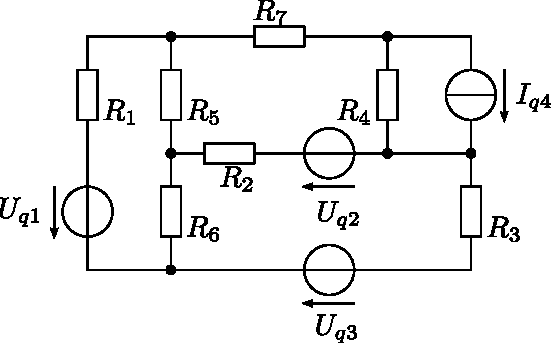
\includegraphics[scale=\schscale]{knotpot_sch.pdf}
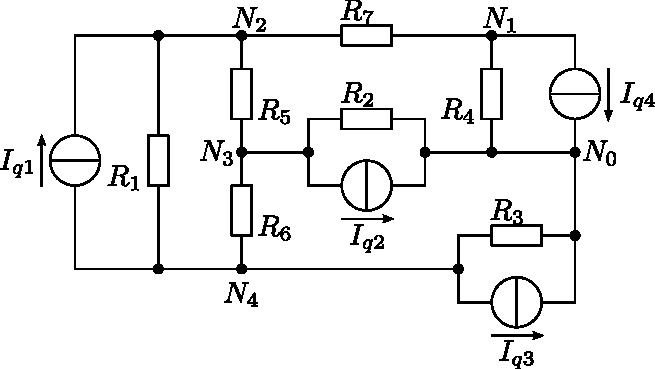
\includegraphics[scale=\schscale]{knotpot_sch_2.pdf}
\caption{Umwandlung von Strom- zu Spannungsquellen}
\label{sch:knotpot_2}
\end{figure}

\begin{table}[h!]
\footnotesize
\[ 	\begin{array}{c|cccc||c}
	N & U_{10}						& U_{20}										& U_{30} 											& U_{40} 											& I \\
	\hline &&&&& \\
	N_1	& \frac{1}{R_4} + \frac{1}{R_7}		& -\frac{1}{R_7} 								& 0 												& 0 												& -I_{q4} 			\\
	&&&&& \\
	N_2	& -\frac{1}{R_7} 					& \frac{1}{R_1} + \frac{1}{R_5} + \frac{1}{R7} 	& -\frac{1}{R_5} 									& -\frac{1}{R_1} 									& I_{q1} 			\\ 
	&&&&& \\
	N_3	& 0 								& -\frac{1}{R_5} 								& \frac{1}{R_2} + \frac{1}{R_5} + \frac{1}{R_6} 	& -\frac{1}{R_6} 									& -I_{q2} 			\\ 
	&&&&& \\
	N_4 & 0 								& -\frac{1}{R_1} 								& -\frac{1}{R_6} 									& \frac{1}{R_1} + \frac{1}{R_3} + \frac{1}{R_6} 	& -I_{q2} -I_{q3} 	\\ 
	&&&&& \\
	\end{array}
\]
\normalsize
\caption{Matrix zu Abb.~\ref{sch:knotpot_2}}
\end{table}

\newpage
     % Knotenpotentialverfahren
% coding:utf-8

%FOSAET, a LaTeX-Code for a electrical summary of basic electronics
%Copyright (C) 2013, Daniel Winz, Ervin Mazlagic

%This program is free software; you can redistribute it and/or
%modify it under the terms of the GNU General Public License
%as published by the Free Software Foundation; either version 2
%of the License, or (at your option) any later version.

%This program is distributed in the hope that it will be useful,
%but WITHOUT ANY WARRANTY; without even the implied warranty of
%MERCHANTABILITY or FITNESS FOR A PARTICULAR PURPOSE.  See the
%GNU General Public License for more details.
%----------------------------------------

\section{Maschenstromverfahren}

\begin{itemize}
	\item Alle realen Quellen in Spannungsquellen wandeln
	\item Maschen legen und nummerieren ($M_1$, $M_2$, $M_3$ ...$M_n$)
	\item Baum bilden (Baum bedeutet hier ein Strang, welcher alle Knoten berührt und durchgehend verbunden ist. Dieser muss keine \textit{Schlange} darstellen, sondern darf auch sternförmig etc. sein.
	\item Matrix aufstellen
	\item Links alle Maschen auflisten
	\item Oben alle Ströme der Quellen eintragen welche zwischen Knoten liegen (nicht jener die innerhalb des Baumes liegen)
	\item Hauptdiagonale ausfüllen:\\ Hierzu sind alle Widerstandswerte zu summieren welche in entsprechender Masche liegen.
	\item Restliche Matrix ausfüllen:\\ Hierzu sind alle Widerstandswerte einzutragen welche zu zwei Maschen gehören einzutragen. Das Vorzeichen ist positiv zu wählen, falls die Maschenpfeilrichtung die selbe ist, sonst negativ.
	\item In der rechten Spalte Spannungsquellen eintragen. Das Vorzeichen ist dabei positiv, falls die Maschenpfeilrichtung entgegen der Spannungspfeilrichtung ist, sonst negativ.
\end{itemize}

\newpage

\subsection{Beispiel}
\begin{figure}[h!]
\centering
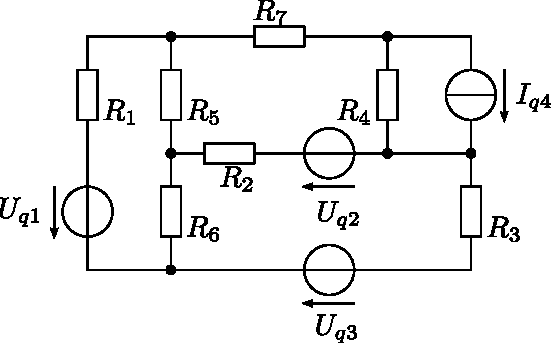
\includegraphics[scale=\schscale]{../fig/mastro_sch.pdf}

\vspace{5mm}

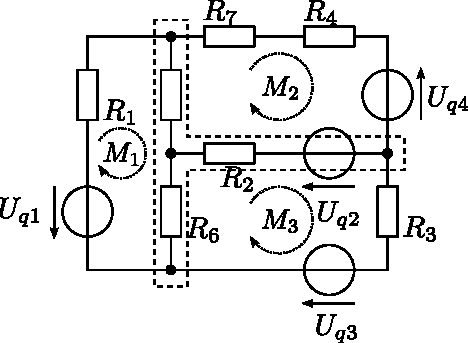
\includegraphics[scale=\schscale]{../fig/mastro_sch_2.pdf}
\caption{Schaltung zum Maschenstromverfahren}
\label{sch:mastro}
\end{figure}

\begin{table}[h!]
\footnotesize
\[ \begin{array}{c|ccc||c}

M	& I_1 & I_2 & I_3 & U \\
\hline &&&& \\
M_1 	& R_1 + R_5 + R_6 	& -R_5 				& -R_6 			& U_{q1} \\
&&&& \\
M_2 	& -R_5 			& R_2 + R_4 + R_5 + R_7 	& -R_2 			& U_{q4} \\
&&&& \\
M_3 	& -R_6 			& -R_2 				& R_2 + R_3 + R_6 	& -U_{q3} \\
\end{array}
\]
\normalsize
\caption{Matrix zu Abb.~\ref{sch:mastro}}
\end{table}
      % Maschenstromverfahren
